
%(BEGIN_QUESTION)
% Copyright 2010, Tony R. Kuphaldt, released under the Creative Commons Attribution License (v 1.0)
% This means you may do almost anything with this work of mine, so long as you give me proper credit

A heat exchanger is used to pre-heat a flow of liquid acetone before it enters a process reactor.  The heating medium is steam, entering the exchanger at 160 PSIA and 480 $^{o}$F, then leaving the exchanger at 120 PSIA and 400 $^{o}$F:

$$\includegraphics[width=15.5cm]{i03974x01.eps}$$

Assuming a steam flow rate of 10 pounds per minute, an acetone flow rate of 25 pounds per minute, and no heat lost to the surrounding environment, calculate:

\vskip 10pt

\begin{itemize}
\item{} The rate of heat exchanged between the steam and the acetone, in BTU/hour (hint: use the enthalpy values found in a {\it steam table})
\vskip 20pt
\item{} The exiting temperature of the acetone, assuming $c$ = 0.521
\end{itemize}

\vfil 

Hint: the {\it Socratic Instrumentation} website contains a page where you may download public-domain textbooks, one of which is a set of steam tables published in 1920.  The {\it Fisher Control Valve Handbook} also has a (less comprehensive) set of steam tables in the Appendix section.

\underbar{file i03974}
\eject
%(END_QUESTION)





%(BEGIN_ANSWER)

This is a graded question -- no answers or hints given!

%(END_ANSWER)





%(BEGIN_NOTES)

The enthalpy of 160 PSIA steam at 480 $^{o}$F is approximately 1260 BTU per pound.  The enthalpy of 120 PSIA steam at 400 $^{o}$F is approximately 1223 BTU per pound.  Both figures come from a {\it superheated steam} table rather than a {\it saturated steam} table, due to the fact that both flows represent steam at temperatures significantly greater than the boiling points at those pressure values.  As the steam expands and cools from its initial state to its final state, the heat liberated per pound is 1260 $-$ 1223 = 37 BTU per pound.

\vskip 10pt

At a steam flow rate of 10 pounds per minute, this equates to a heat transfer rate of 370 BTU per minute, or {\bf 22,200 BTU per hour}.

\vskip 10pt

With acetone flowing at 25 pounds per minute, and the steam delivering 370 BTU per minute of heat to the acetone, this means each pound of acetone receives a heat input of 14.8 BTU.  Calculating the temperature rise for the acetone:

$$Q = mc \Delta T$$

$$\Delta T = {Q \over mc} = {14.8 \over (1)(0.521)} = 28.4^o \hbox{F}$$

Since we are told the acetone enters the heat exchanger at 40 $^{o}$F, and we now know it rises in temperature by 28.4 $^{o}$F, the exiting acetone temperature must be {\bf 68.4 $^{o}$F}.

%INDEX% Physics, heat and temperature: calorimetry problem (with latent heat) 
%INDEX% Physics, heat and temperature: steam table

%(END_NOTES)


